\documentclass{article}
\usepackage{iclr2027_conference,times}
% Keep the official anonymous review format; enable only for an accepted paper.
% \iclrfinalcopy
\usepackage{amsmath,amssymb,amsfonts}
\usepackage{graphicx}
\usepackage{textcomp}
\usepackage{xcolor}
\usepackage{booktabs}
\usepackage{multirow}
\usepackage{needspace}
% Two-line table header on a common baseline with single-line headers.
% \shortstack centres vertically, which leaves stacked and unstacked headers
% sitting on different baselines in the same row.
\newcommand{\hdr}[2]{\begin{tabular}[b]{@{}c@{}}\textbf{#1}\\\textbf{#2}\end{tabular}}
\newcommand{\thead}[1]{\textbf{\shortstack[b]{#1}}}
\usepackage[hyphens]{url}
% Long URLs in the footnote and bibliography cannot break at "/" or "." under
% the url package alone, which leaves the surrounding line badly underfull.
\usepackage{xurl}
\usepackage[hidelinks]{hyperref}

\begin{document}

\title{LaDiM: Layered Diagnosis for\\
Multi-Agent Code Migration}

\author{Anonymous Authors}

\maketitle

\begin{abstract}
Migrating deep learning training code across frameworks requires preserving
training behavior. Large language models can produce executable translations
whose forward values agree with the source, yet whose gradients or parameter
updates are incorrect. Checking these stages exposes such faults, but error
propagation can produce multiple discrepancies and obscure which computation
needs repair. We propose LaDiM, a multi-agent repair system that uses
dependencies between training stages to organize verification evidence into
layered diagnoses. Its verifier compares execution status, forward values,
gradients, and parameter updates in training order, and reports the first
failing stage together with the supporting measurements. The translator
supplies an initial target program, and the repair agent uses this diagnosis
to edit the permitted code. An orchestrator coordinates translation,
verification, and repair, using updated diagnoses after each edit to guide
subsequent attempts within a fixed budget. On 50 MindSpore fault instances,
LaDiM achieves full acceptance within four attempts, with 84\% accepted on
the first attempt and approximately 29-fold lower token cost per accepted
repair than the strongest state-of-the-art baseline tested.
Experiments on MindSpore and JAX demonstrate the effectiveness of the same
diagnosis and repair procedure across target frameworks.
\end{abstract}

\section{Introduction}

Migrating deep learning training code makes existing programs available in another framework and its software and hardware ecosystem. Large language models (LLMs) reduce the manual effort involved in code translation~\citep{he-etal-2025-execoder,macedo2024intertrans}, but an executable translation may still change how a model learns. A PyTorch program moved to MindSpore or JAX can produce different forward values, compute incorrect gradients despite matching losses, or update the wrong parameters despite plausible gradients. Differences in operator conventions, differentiation interfaces, and optimizer semantics cause these failures~\citep{paszke2019pytorch,mindspore2020whitepaper,google2025torchax}. Preserving training behavior requires checking each computation and identifying where a discrepancy originates.

\begin{figure}[t]
\centering
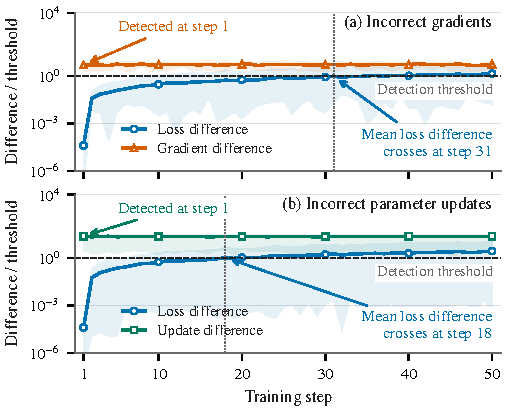
\includegraphics[width=\linewidth]{figures/gradient_drift.pdf}
\caption{Loss and gradient differences (a) and loss and update differences (b), normalized by each signal's threshold. Gradient and update checks detect faults at step~1 in all 12 runs per panel. The mean loss difference crosses the detection threshold (dashed) at steps 31 and 18, respectively. Curves show means and shading shows ranges.}
\label{fig:gradient-drift}
\end{figure}

The evidence available to translation and repair systems does not directly identify this origin. Unit tests check translated behavior~\citep{roziere2021unittests}; interactive agents inspect code and execution results~\citep{yang2024sweagent}; RepoTransAgent combines repository context, test failures, and reflection~\citep{guan2025repotransagent}; and MatchFixAgent supplies reports from multiple semantic analyses to guide test generation and repair~\citep{ibrahimzada2025matchfixagent}. These approaches leave the repair process to infer how discrepancies depend on one another during training. A forward error can change both gradients and parameter updates, while an incorrect update affects later forward computations as training continues. Figure~\ref{fig:gradient-drift} shows the resulting delay: the gradient or parameter update check detects every injected fault at step~1, whereas the mean loss difference crosses its threshold only at steps 31 and 18 in panels (a) and (b). The faulty computation is observable well before its accumulated effect on loss. We use these dependencies to interpret verification results in training order. Execution must succeed before numerical comparisons are available; once forward values agree, later discrepancies direct attention to differentiation or optimizer behavior. Selecting the first failing stage gives the repair agent a computation to inspect even when several measurements disagree.

We introduce LaDiM (Layered Diagnosis for Multi-Agent Code Migration), which reports this stage together with its supporting measurements as a layered diagnosis. A translator supplies the initial target program, a verifier produces the diagnosis, and a repair agent uses it to edit the affected code. An orchestrator coordinates these agents and updates the diagnosis after each edit. Experiments on MindSpore and JAX examine repair effectiveness, diagnostic accuracy, and feedback design. On the 50-instance MindSpore set, LaDiM achieves full acceptance within four attempts with approximately 29-fold lower token cost per accepted repair than MatchFixAgent. This paper makes three contributions.

\begin{itemize}
  \item We formulate training-code repair through diagnosis along ordered training computations, using the first failing stage to connect verification evidence with a repair target.
  \item We develop LaDiM, a layered multi-agent repair framework in which an orchestrator coordinates specialized translator, verifier, and repair agents around this diagnosis.
  \item We evaluate repair effectiveness and cross-framework applicability on MindSpore and JAX, and analyze diagnostic accuracy, signal coverage, and guidance for the failing stage.
\end{itemize}

\section{Related Work}

\paragraph{Code Translation and Framework Migration.}
Neural translation methods learn code mappings from multilingual corpora and incorporate automated tests or compiler representations to improve translations~\citep{roziere2020transcoder,roziere2021unittests,szafraniec2023compiler}. ExeCoder encodes functional semantics, syntax structure, and variable dependencies~\citep{he-etal-2025-execoder}; InterTrans explores intermediate translation paths~\citep{macedo2024intertrans}; and RepoTransAgent uses repository context, test failures, and reflection to refine translated code~\citep{guan2025repotransagent}. Framework migration tools supply mappings between programming interfaces: MindConverter targets MindSpore~\citep{mindspore2023mindconverter}, Ivy\footnote{\url{https://github.com/unifyai/ivy}} and \texttt{torch2jax}\footnote{\url{https://github.com/rdyro/torch2jax}} convert computations to JAX, and TorchAX exposes the PyTorch interface over a JAX backend~\citep{google2025torchax}. Executable translations can still compute incorrect forward values, gradients, or parameter updates. LaDiM addresses these training faults through semantic repair of both the translated program and the compatibility-layer implementations on which it depends.

\paragraph{Differential Testing and Deep Learning Verification.}
Differential testing exposes compiler and program faults through disagreement between related executions~\citep{yang2011csmith,le2014emi}. DeepXplore combines neuron coverage with differences between the outputs of functionally similar networks to search for inputs that expose erroneous behavior~\citep{pei2017deepxplore}. DeepGauge develops testing criteria at multiple granularities to assess how thoroughly a test set exercises a deep learning system~\citep{ma2018deepgauge}. These studies examine test adequacy and behavioral differences, providing ways to select inputs and identify inconsistent observations. Cross-framework training repair also requires interpreting the dependencies between observations: a forward error can propagate to gradients and parameter updates, so several discrepancies may originate from one faulty computation. LaDiM turns these measurements into a layered diagnosis by checking execution, forward values, gradients, and parameter updates in training order. The first failing stage and its supporting measurements identify the computation to inspect, connecting differential verification to a repair target.

\paragraph{Automated Program Repair and LLM Agents.}
Automated program repair uses tests or semantic constraints to guide patch generation~\citep{nguyen2013semfix}, and pretrained language models generate patches from code and failure evidence~\citep{xia2023aprplm}. Interactive agents extend this process through repository navigation, editing, and execution, as in SWE-agent~\citep{yang2024sweagent}, or through reflection, self-debugging, and executable code actions~\citep{shinn2023reflexion,chen2023selfdebugging,wang2024codeact}. Multi-agent systems distribute these activities among specialized roles: ChatDev and MetaGPT organize software development~\citep{qian2023chatdev,hong2023metagpt}, while AutoGen and AgentVerse support agent communication and cooperation~\citep{wu2023autogen,chen2023agentverse}. For translation repair, MatchFixAgent combines semantic validation with autonomous patch generation~\citep{ibrahimzada2025matchfixagent}. Its analyzers examine control flow, data flow, input and output behavior, libraries, exceptions, and specifications; their reports guide test generation, patching, and equivalence judgments. This decomposition organizes verification by semantic aspect. LaDiM organizes the repair loop around dependencies between training computations, using the layered diagnosis as the interface between translation, verification, and repair agents. After each edit, the orchestrator obtains a new diagnosis and uses the first failing stage and its measurements to guide the next repair.

\section{Method}

% Place the overview near the method description in the single-column layout.
\begin{figure}[!t]
\centering
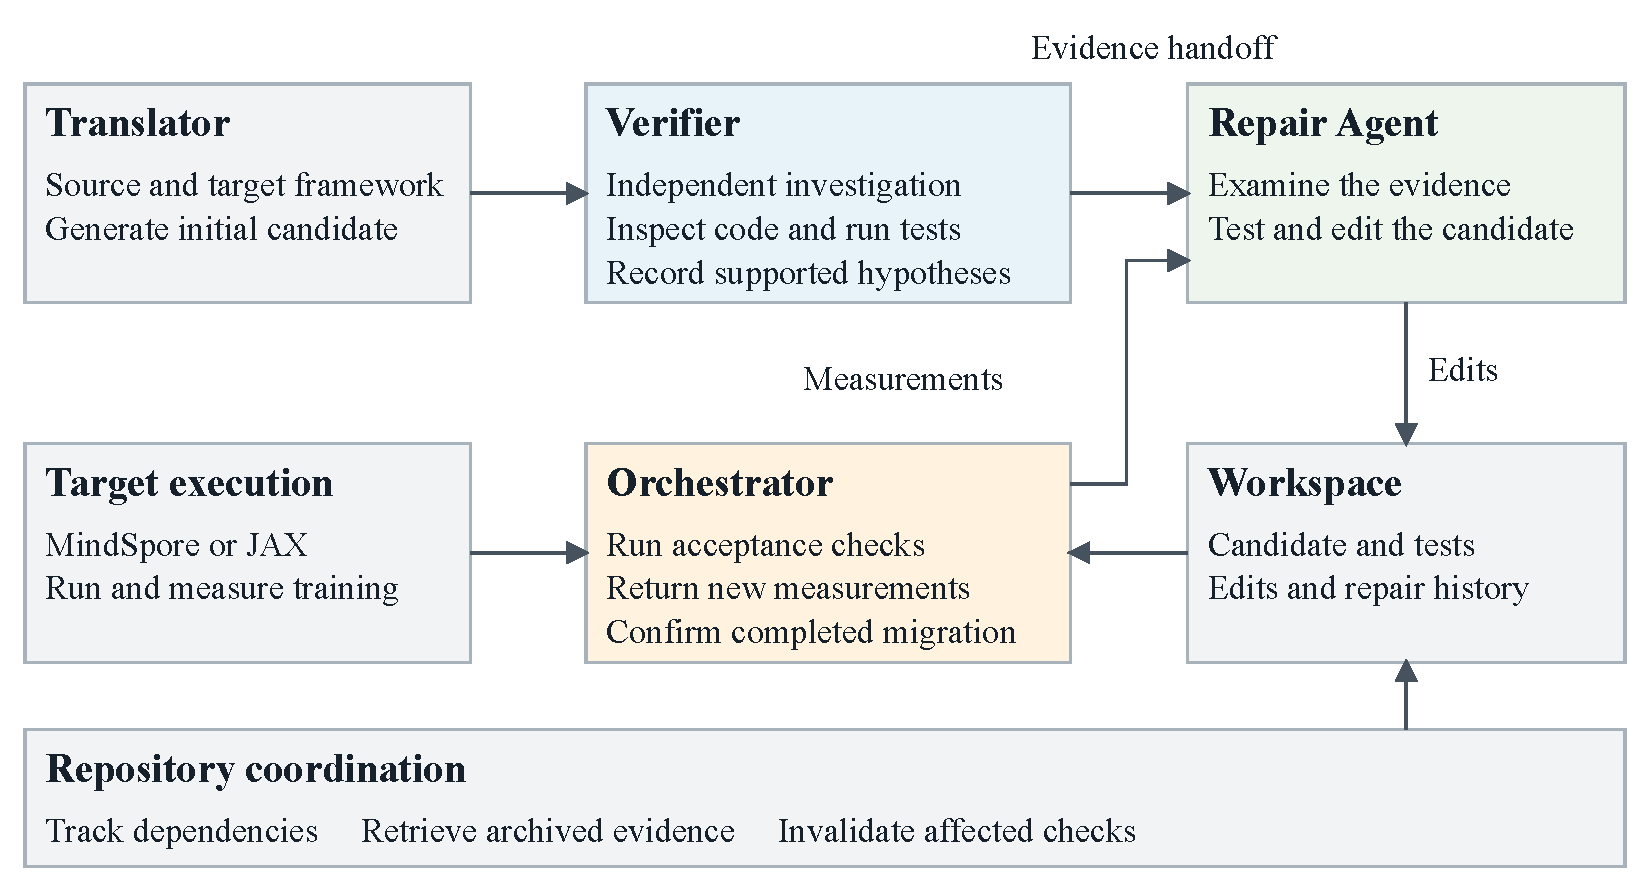
\includegraphics[width=\textwidth]{figures/hierarchical_feedback_architecture.pdf}
\caption{LaDiM's repair loop. An orchestrator coordinates the translator, verifier, and repair agents. The verifier's diagnosis guides edits to the permitted code, followed by verification of the updated program. The \texttt{torch4ms}/MindSpore and TorchAX/JAX implementations use the same diagnostic signals and repair procedure.}
\label{fig:architecture}
\end{figure}

\subsection{Problem Setup}
Given a training program $P$ in a source framework $F_s$ and a target framework $F_t$, migration produces a target program $\hat{P}$ that preserves the source's training computations. We examine execution, forward values, gradients, and parameter updates. The repair task takes the source program, an initial target implementation, and the code the repair agent is permitted to edit. It returns a revised implementation that passes the specified verification checks. The permitted code can include the translated program or the framework implementation needed to execute it. The verifier runs the source and target programs with controlled inputs, synchronized initialization, and matched optimizer settings. Let $\mathcal{O}_{t}(P)$ denote the observations at training step $t$, including execution status, selected outputs or losses, gradients, and parameter updates. Differences between $\mathcal{O}_{t}(P)$ and $\mathcal{O}_{t}(\hat{P})$ provide the evidence for diagnosis. Section~\ref{sec:setup} specifies the checked conditions, tolerances, and repair acceptance criteria used in the experiments.

\subsection{Layered Diagnosis}
LaDiM interprets verification evidence in the order required by training computation. Execution failures prevent numerical comparison. A discrepancy in forward computation can propagate to gradients and parameter updates, so several failing measurements may reflect the same earlier error. When forward values agree, discrepancies in gradients or parameter updates direct attention to differentiation or optimizer behavior. We select the stage that fails first. Let $\mathcal{C}=(c_1,c_2,c_3)$ be the ordered diagnostic signals for execution, forward values, and gradients and parameter updates. Let $\mathrm{fail}(\hat{P})\subseteq\mathcal{C}$ contain the signals that detect a failure in the target implementation. LaDiM identifies the first failing stage,
\begin{equation}
v_{\mathrm{LaDiM}}(\hat{P}) =
\begin{cases}
\min\left\{\, i : c_i \in \mathrm{fail}(\hat{P}) \,\right\}, & \mathrm{fail}(\hat{P}) \neq \emptyset,\\
\text{verified}, & \text{otherwise},
\end{cases}
\end{equation}
and reports the measurements, available module locations, and exception details that support this choice. The selected stage and this evidence form the layered diagnosis. Supplied with the editable code, they guide repair toward execution compatibility or operator implementation at index 1, forward operator semantics at index 2, and differentiation, parameter registration, or optimizer behavior at index 3. Later signals can still provide supporting evidence for the edit.

\subsection{Diagnostic Signals}
\label{sec:hierarchy}

The execution signal checks whether $\hat{P}$ completes the training step under the target runtime. When execution fails, it records the operation, exception, and location available from the run. Failures can occur during module construction, data movement, forward computation, loss computation, backward computation, or parameter updates. These observations direct repair toward compatibility, operator implementation, device placement, data type, shape, or parameter registration. Numerical measurements are unavailable after an execution failure. Omitting a backward call can pass the execution check, leaving missing gradients and parameter updates to be detected by the third signal.

Once both executions complete, the signal for forward values compares logits, selected intermediate activations, and losses under controlled inputs $(x,y)$ and synchronized initialization. The simplest comparison uses the loss difference,
\begin{equation}
\Delta_{\mathrm{loss}} =
\left| L(P; x, y) - L(\hat{P}; x, y) \right|.
\end{equation}
When intermediate outputs are available, the verifier also locates the earliest module whose difference exceeds tolerance. This helps locate mismatches in operators, reductions, broadcasting, normalization, or loss computation that would otherwise appear only in the final loss. Agreement here leaves backward computation and optimizer behavior to be checked by the gradient and parameter update signal. The verifier measures differences in gradient norms and relative differences in parameter updates using
\begin{equation}
\Delta_{\mathrm{grad}} =
\left|
\|\nabla_{\theta} L(P)\|_2 -
\|\nabla_{\hat{\theta}} L(\hat{P})\|_2
\right|,
\end{equation}
\begin{equation}
\Delta_{\mathrm{param}} =
\frac{\|\Delta \theta - \Delta \hat{\theta}\|_2}
{\|\Delta \theta\|_2 + \epsilon}.
\end{equation}
Here $\Delta\theta$ and $\Delta\hat{\theta}$ are the source and target parameter updates, and $\epsilon$ prevents division by zero. The verifier also records missing gradients, parameters with zero gradients, mismatches in parameter names, and update outliers. Missing target gradients for parameters differentiated in the source direct attention to automatic differentiation or parameter registration. Matching gradient measurements with divergent parameter updates direct attention to optimizer behavior.

\subsection{Multi-Agent Repair}

The translator in Figure~\ref{fig:architecture} receives the source program and target framework information and produces the initial target program. The verifier runs the paired executions, and the repair agent uses the resulting diagnosis, the permitted code, and feedback from the previous attempt to edit the failing computation. The orchestrator maintains the program state and attempt budget, invoking verification after each edit. If an edit improves the verification score, it is retained; otherwise, the orchestrator rolls it back. The next attempt receives the updated diagnosis and the preceding edit's outcome, so a change in the failing stage redirects repair to the newly implicated computation. The loop ends when verification succeeds or the budget is exhausted.

The verifier collects observations through execution adapters. The primary adapter, \texttt{torch4ms}, exposes the PyTorch interface and dispatches operators, backward computation, and optimizer behavior to MindSpore implementations.\ificlrfinal\footnote{The primary prototype repository is available at \url{https://gitee.com/feixiao13/ascend-torch4ms.git}.}\fi{} The second uses TorchAX with JAX automatic differentiation and Optax updates. Both return execution status, forward values, gradients, and parameter updates in a common format, so the same diagnosis and repair procedure applies to both targets.

\section{Experiments}

\subsection{Experimental Setup}
\label{sec:setup}
We constructed the repair set from failures recorded while migrating PyTorch training programs to MindSpore and JAX. The failures fall into 25 recurring categories: ten cause execution failures, seven affect forward values, and eight affect gradients or parameter updates. The latter 15 leave the program executable. We reproduce each category by injecting the observed fault into a correct implementation, giving it a known location for evaluating diagnosis and reducing the variation in failures collected directly from migrations. Instantiating each category on two model families yields 50 instances across CNN, image MLP, Transformer classifier, and tiny causal LM. The JAX set uses the same construction for six MLP and CNN faults across the three stages. We also identify the code that must change to correct each fault. Depending on this repair location, the permitted edits cover the translated program, additionally include operator implementations in the compatibility layer, or extend to that layer's automatic differentiation and optimizer code. We restrict each repair to its permitted code because an edit above the fault can hide its effect while leaving the faulty implementation unchanged.

We compare LaDiM with direct LLM repair, SWE-agent, and MatchFixAgent, and examine reduced feedback configurations in Section~\ref{sec:ablations}. The main MindSpore comparison uses the same faulty translations, LLM (\texttt{deepseek-v4-flash}), temperature (0.1), and four-attempt budget. MatchFixAgent also receives the correct implementation of the changed function, a reference supplied only to that baseline. The JAX comparison uses the same LLM and includes Ivy and \texttt{torch2jax}; LaDiM has up to three repair rounds, while Direct LLM and each conversion tool run once. On the 50-instance set, acceptance means passing the checks specific to the injected fault, and we report it after one attempt and within four attempts. The diagnostic studies separately check that every measured source--target difference stays within its threshold at every training step: $\Delta_{\mathrm{loss}}\leq0.02$, $\Delta_{\mathrm{grad}}\leq0.05$, and $\Delta_{\mathrm{param}}\leq0.03$, as defined in Section~\ref{sec:hierarchy}. We record edits outside the permitted code and measure cost across all attempted instances, including unsuccessful repairs. Tokens per accepted repair divide total prompt and completion tokens by the accepted count; elapsed time uses the same denominator. These studies use controlled executions; longer training runs and additional framework pairs remain for future evaluation.

\subsection{Repair Effectiveness and Efficiency}
\label{sec:main-results}

\begin{table}[!htb]
\caption{Repair acceptance and cost on MindSpore and JAX. Each panel uses its own instance set and recorded attempt budget.}
\label{tab:main-results}
\centering
\small
\setlength{\tabcolsep}{4pt}
\renewcommand{\arraystretch}{1.1}
\begin{tabular*}{\linewidth}{@{\extracolsep{\fill}}lrrrr@{}}
\toprule
\textbf{Method} & \thead{Accepted\\repairs} & \thead{First-attempt\\acceptance} & \thead{Tokens per\\accepted repair} & \thead{Seconds per\\accepted repair} \\
\midrule
\multicolumn{5}{l}{\textit{(a) MindSpore: 50 instances, up to four attempts}} \\
% Generated from the original Fixed50 summary.
Direct LLM & 40/50 & 72\% & 39.6K & 54.2 \\
SWE-agent & 46/50 & 72\% & 166.0K & 138.6 \\
MatchFixAgent$^\dagger$ & 47/50 & 74\% & 110.7K & 74.2 \\
\textbf{LaDiM} & \textbf{50/50} & \textbf{84\%} & \textbf{3.8K} & \textbf{21.8} \\
\midrule
\multicolumn{5}{l}{\textit{(b) JAX: six instances, all accepted repairs finish in the first round}} \\
% Generated by figures/make_jax_table.py; do not edit the numbers.
Direct LLM & 5/6 & 83.3\% & 15.0K & 177.1 \\
Ivy & 0/6 & 0.0\% & n/a & n/a \\
\texttt{torch2jax} & 0/6 & 0.0\% & n/a & n/a \\
\midrule
\textbf{LaDiM} & \textbf{6/6} & \textbf{100.0\%} & \textbf{2.9K} & \textbf{79.8} \\
\bottomrule

\end{tabular*}
\par\vspace{4pt}
\begin{minipage}{\linewidth}
\footnotesize MindSpore acceptance uses the checks for each injected fault. JAX acceptance requires training verification on three seeds for each instance; its six instances cover MLP and CNN at all three fault stages, with edits confined to the translated program. LaDiM permits up to three repair rounds on JAX, while Direct LLM, Ivy, and \texttt{torch2jax} run once. Costs sum all attempted instances, including failures, and divide by accepted repairs; n/a denotes an undefined cost when no repair is accepted. $^\dagger$Only MatchFixAgent receives the correct implementation of the changed function.
\end{minipage}
\end{table}
LaDiM repairs all 50 MindSpore instances within four attempts, with 84\% accepted on the first attempt compared with 74\% for MatchFixAgent (Table~\ref{tab:main-results}). The repair-location breakdown in Appendix~\ref{sec:repair-breakdown} places its remaining advantage over the external repair systems in adapter code: SWE-agent and MatchFixAgent resolve every fault confined to the translated program but miss faults in automatic differentiation or optimizer implementations. Here a program may execute and produce a plausible loss while relating gradients to parameters incorrectly. LaDiM resolves all four such instances, including one missed by every baseline. The cumulative results in Figure~\ref{fig:repair-comparison} show that most repairs require little iteration: LaDiM approaches full acceptance by the second attempt and resolves the last instance within four. It also uses approximately 29-fold fewer tokens and 3.4-fold less elapsed time per accepted repair than MatchFixAgent, with both measures counting unsuccessful attempts. The combination of higher first-attempt acceptance and lower total cost motivates the comparison of diagnosis and repair guidance in Section~\ref{sec:ablations}.

\begin{figure}[t]
\centering
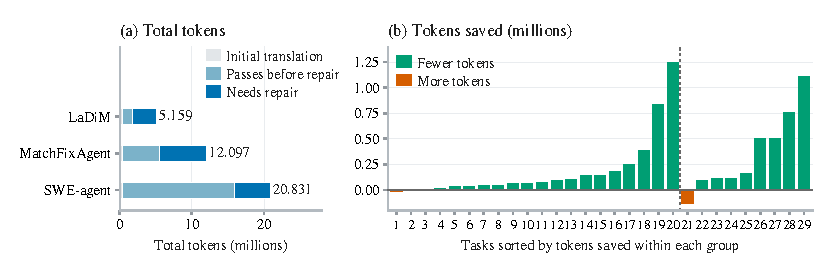
\includegraphics[width=\textwidth]{figures/repair_comparison.pdf}
\caption{Repair cost and acceptance on the 50 MindSpore instances. (a) First-attempt acceptance versus total tokens divided by repairs accepted within four attempts. (b) Cumulative acceptance at the recorded budgets of one, two, and four attempts; connecting lines are visual guides. All six curves use the original MindSpore experiment in Table~\ref{tab:main-results}(a) and Appendix~\ref{sec:repair-breakdown}.}
\label{fig:repair-comparison}
\end{figure}

\subsection{Generalization Across Frameworks}
\label{sec:generalization}

The same diagnosis and repair procedure applies to JAX in Table~\ref{tab:main-results}(b). LaDiM repairs all six faults across execution, forward values, and gradients and parameter updates; its additional accepted repair over Direct LLM corrects forward computation in the CNN. All accepted repairs finish in the first round. LaDiM uses 2.9K tokens per accepted repair compared with 15.0K for Direct LLM. The adapter collects observations through the JAX runtime, and the verifier interprets them in the same training order used for MindSpore.

\subsection{Diagnosis Analysis}
\label{sec:fault-characterization}

The diagnostic signals distinguish the effects of faults along the training computation. Correct reference translations of CNN, MLP, Transformer, and tiny causal LM models pass every check over 50 steps and three seeds: the maximum loss difference is $3.815\times10^{-6}$, and mean differences in gradient norms and parameter updates remain below $4\times10^{-8}$ and $3.9\times10^{-6}$. We isolate injected faults by synchronizing the translated model with the source at each checked step, again using 50 steps, four model families, and three seeds. The intended signal detects all 36 faults across the three classes. Execution failures leave numerical measurements unavailable; forward faults cross the loss threshold and can also affect gradients and updates; gradient faults preserve loss agreement but affect gradients and updates; and update faults affect only the update comparison. The tiny causal LM further shows why the measurements are complementary: its forward fault crosses the loss threshold even though the gradient signal stays below threshold. Selecting the first failing stage localizes 48 of 50 instances correctly (96\%), including all execution faults (20/20) and all gradient and parameter update faults (16/16). The two disagreements with the injected-stage labels arise from mixed precision overflow: execution fails before forward values can be compared, so the diagnosis reports the execution failure.

Allowing the translated model to retain its own state exposes a different consequence of the same dependencies. Incorrect updates accumulate and change later forward computations in Figure~\ref{fig:gradient-drift}. Across four model families and three seeds for each of two fault types (24 runs), gradient or parameter update checks detect the fault immediately, while the mean loss difference crosses its threshold only after further training. Forward agreement can therefore persist while incorrect gradients or updates already affect learning.

\Needspace{12\baselineskip}
\subsection{Ablation Study}
\label{sec:ablations}

We examine how signal coverage and diagnostic feedback affect repair. The signal study uses 12 tasks spanning the three fault stages and four model families. The feedback ablation uses the 50 MindSpore instances with the faulty programs, repair LLM, permitted edits, and four-attempt budget fixed. Execution only supplies runtime feedback; pass/fail only compresses all checks into one decision; stage label only identifies the first failing stage; and flat feedback supplies all measurements without stage selection or targeted repair guidance. Table~\ref{tab:feedback-ablation} compares their repair acceptance and cost with the full method.

\begin{table}[!htb]
\caption{Effect of diagnostic feedback on repair acceptance and cost across 50 MindSpore instances.}
\label{tab:feedback-ablation}
\centering
\small
\setlength{\tabcolsep}{4pt}
\renewcommand{\arraystretch}{1.1}
\begin{tabular*}{\linewidth}{@{\extracolsep{\fill}}lrrrr@{}}
\toprule
\textbf{Variant} & \thead{Accepted\\repairs} & \thead{First-attempt\\acceptance} & \thead{Tokens per\\accepted repair} & \thead{Seconds per\\accepted repair} \\
\midrule
% Generated from the feedback-ablation results.
\textbf{LaDiM}$^\ast$ & 48/50 & 72\% & 6.8K & 100.2 \\
\midrule
Execution only & 33/50 & 64\% & 7.2K & 251.0 \\
Pass/fail only & 34/50 & 64\% & 22.0K & 410.7 \\
Stage label only & 34/50 & 64\% & 18.5K & 341.6 \\
Flat feedback & 34/50 & 64\% & 12.7K & 357.2 \\
\midrule
Without targeted guidance & -- & -- & -- & -- \\
Without repair history & -- & -- & -- & -- \\
Without rollback & -- & -- & -- & -- \\
\bottomrule

\end{tabular*}
\par\vspace{4pt}
\begin{minipage}{\linewidth}
\footnotesize All variants use \texttt{deepseek-v4-flash} at temperature 0 and paired-threshold acceptance within four attempts. Costs include unsuccessful attempts. $^\ast$LaDiM reports the third of three independent runs; all three results appear in Appendix~\ref{sec:feedback-evidence}. -- denotes an unmeasured result. The last three variants each disable the named component while retaining the remaining procedure.
\end{minipage}
\end{table}

Complementary signals make faults at successive training stages visible to repair. Adding forward comparisons to execution feedback raises acceptance from 4/12 to 8/12; adding gradient and parameter update feedback raises it to 12/12. Each setting repairs the four faults at each visible stage, and every accepted repair finishes in the first round (Table~\ref{tab:signal-coverage}).

Combining measurements with stage selection and targeted guidance improves both repair acceptance and efficiency. LaDiM accepts 48/50 repairs, compared with 34/50 under flat feedback, while reducing tokens per accepted repair from 12.7K to 6.8K and elapsed time from 357.2 to 100.2 seconds. Its first-attempt acceptance also rises from 64\% to 72\%. The stage-label condition reaches the same acceptance as flat feedback at a higher token cost. LaDiM gives the repair agent both the measurements behind the selected stage and guidance on the implicated computation.

Framework documentation has a different role (Appendix~\ref{sec:framework-documentation}). The \texttt{torch4ms} usage guides enable initial translations to complete training in all 15 runs, compared with none without them. During repair, the guides eliminate out-of-scope operator edits but leave operator acceptance unchanged, reduce acceptance for translated-program faults, and leave automatic differentiation and optimizer faults unresolved. Their benefit in supplying interface conventions during translation does not carry over consistently to repair.

\section{Conclusion}

We introduced LaDiM, a multi-agent repair system that uses the order of training computations to diagnose migration failures. The first failing stage connects verification evidence to a computation that requires correction, including faults that remain hidden in forward observations. LaDiM turns this diagnosis into code edits through specialized translation, verification, and repair agents coordinated by an orchestrator. Experiments on MindSpore and JAX show improved repair acceptance and lower token cost with the same diagnosis and repair procedure across target frameworks.

% Required by ICLR 2027; left blank at the author's request.
\subsection*{AI use statement}

\ificlrfinal
\subsubsection*{Acknowledgments}
This work was supported by CAAI Huawei MindSpore Open Fund, and developed on OpenI Community.
\fi

\bibliographystyle{iclr2027_conference}
\bibliography{ref}

\clearpage
\appendix
\section{Framework Documentation Studies}
\label{sec:framework-documentation}

The \texttt{torch4ms} usage guides describe framework interfaces, operator conventions, and optimizer usage. We first evaluate them as repair context on 24 CNN and MLP tasks requiring edits to the translated program, operator code, or automatic differentiation and optimizer code. With the translator fixed, four conditions combine execution-only pass/fail or layered feedback with the repair guide present or absent; each allows four attempts. The task configuration and feedback implementation are separate from the 50-instance comparison in Section~\ref{sec:ablations}. Under layered feedback, documentation eliminates edits outside the permitted operator code without increasing operator acceptance, reduces acceptance for translated-program faults, and leaves automatic differentiation and optimizer faults unresolved (Table~\ref{tab:guidance-ablations}(a)). The diagnoses detect the latter faults, but the edits do not pass acceptance checks. All execution-only pass/fail conditions accept no repairs because executable numerical and gradient faults do not trigger the repair agent under that policy. Comparing these conditions with layered feedback thus changes both which faults trigger repair and what evidence guides an edit.

For initial translation, we disable repair and run five held-out tasks three times per condition. Both conditions use the same source programs, base prompt, target environment, verifier, and \texttt{deepseek-v4-flash} at temperature 0.1, with one translator call per run; only the guide differs. Without it, most programs fail to compile and none completes training. With it, all 15 compile, execute, and produce gradients and parameter updates (Table~\ref{tab:guidance-ablations}(b)), supporting the use of target interface conventions in the translator prompt. Here training completion requires a non-empty gradient and a non-zero parameter update and is measured separately from paired numerical agreement with the source.

\begin{table}[!htb]
\caption{Effect of framework documentation on repair in a separate 24-task study (a) and on translation in a single attempt across five tasks with three repeats each (b).}
\label{tab:guidance-ablations}
\centering
\small
\setlength{\tabcolsep}{4pt}
\renewcommand{\arraystretch}{1.12}
\begin{tabular*}{\linewidth}{@{\extracolsep{\fill}}llcccc@{}}
\multicolumn{6}{l}{\textit{(a) Documentation supplied to the repair agent}} \\
\toprule
\hdr{Code the agent}{may edit} & \thead{Framework\\documentation} & \textbf{Verified} & \hdr{One}{attempt} & \hdr{Four}{attempts} & \hdr{Edits outside}{that code} \\
\midrule
Translated program & Off & 12/12 & 100.0\% & 100.0\% & 0.0\% \\
Translated program & On  & 8/12  & 58.3\%  & 66.7\%  & 0.0\% \\
\addlinespace[3pt]
Operator code & Off & 6/8 & 50.0\% & 75.0\% & 12.5\% \\
Operator code & On  & 6/8 & 50.0\% & 75.0\% & 0.0\% \\
\addlinespace[3pt]
\multirow{2}{*}{\shortstack[l]{Automatic differentiation\\and optimizer code}} & Off & 0/4 & 0.0\% & 0.0\% & 0.0\% \\
 & On  & 0/4 & 0.0\% & 0.0\% & 0.0\% \\
\bottomrule
\end{tabular*}
\par\vspace{7pt}

\setlength{\tabcolsep}{3pt}
\begin{tabular*}{\linewidth}{@{\extracolsep{\fill}}lrrrrr@{}}
\multicolumn{6}{l}{\textit{(b) Framework documentation in the translator, with repair disabled}} \\
\toprule
\thead{Framework\\documentation} & \textbf{Runs} & \textbf{Compile} & \textbf{Execute} & \textbf{Train} & \textbf{All three} \\
\midrule
Off & 15 & 13.3\% & 13.3\% & 0.0\% & 0.0\% \\
On  & 15 & 100.0\% & 100.0\% & 100.0\% & 100.0\% \\
\bottomrule
\end{tabular*}
\par\vspace{4pt}
\begin{minipage}{\linewidth}
\footnotesize On and Off indicate whether the prompt includes the corresponding \texttt{torch4ms} usage guide. Panel (a) shows layered feedback with a four-attempt budget. The last column reports the percentage of repairs that edit code outside the permitted scope. In (b), All three requires compilation, execution, and training completion in one attempt; training completion requires a non-empty gradient and a non-zero parameter update.
\end{minipage}
\end{table}


\clearpage
\section{Repair Results by Fault, Location, and Model}
\label{sec:repair-breakdown}

Table~\ref{tab:repair-breakdown} gives the breakdown underlying the main MindSpore results. Table~\ref{tab:original-feedback} records the execution-only and all-signals conditions from the same run. These results use fault-specific acceptance at temperature 0.1. Figure~\ref{fig:repair-comparison} uses this experiment for every curve.

\begin{table}[!htb]
\caption{Acceptance by fault stage, repair location, and model in the original 50-instance MindSpore experiment.}
\label{tab:repair-breakdown}
\centering
\small
\setlength{\tabcolsep}{4pt}
\renewcommand{\arraystretch}{1.08}
\begin{tabular*}{\linewidth}{@{\extracolsep{\fill}}lcccc@{}}
\toprule
\textbf{Measure} & \textbf{Direct LLM} & \textbf{SWE-agent} & \textbf{MatchFixAgent}$^\dagger$ & \textbf{LaDiM} \\
\midrule
\multicolumn{5}{l}{\textit{Fault stage}} \\
Execution & 18/20 & 20/20 & 20/20 & \textbf{20/20} \\
Forward values & 8/14 & 11/14 & 14/14 & \textbf{14/14} \\
Gradients and parameter updates & 14/16 & 15/16 & 13/16 & \textbf{16/16} \\
\midrule
\multicolumn{5}{l}{\textit{Repair location}} \\
Translated program & 24/26 & 26/26 & 26/26 & \textbf{26/26} \\
Operator code & 14/20 & 17/20 & 20/20 & \textbf{20/20} \\
Automatic differentiation and optimizer & 2/4 & 3/4 & 1/4 & \textbf{4/4} \\
\midrule
\multicolumn{5}{l}{\textit{Model}} \\
CNN & 12/13 & 13/13 & 13/13 & \textbf{13/13} \\
MLP & 7/13 & 11/13 & 12/13 & \textbf{13/13} \\
Transformer & 11/12 & 11/12 & 10/12 & \textbf{12/12} \\
Language model & 10/12 & 11/12 & 12/12 & \textbf{12/12} \\
\bottomrule
\end{tabular*}
\par\vspace{4pt}
\begin{minipage}{\textwidth}
\footnotesize Fractions count accepted repairs over evaluated instances, using the checks for each injected fault in Section~\ref{sec:setup}. All counts use the four-attempt budget. The language model is the tiny causal language model. $^\dagger$Only MatchFixAgent receives the correct implementation of the changed function.
\end{minipage}
\end{table}

\begin{table}[!htb]
\caption{Reduced feedback in the original 50-instance MindSpore experiment used by Figure~\ref{fig:repair-comparison}.}
\label{tab:original-feedback}
\centering
\small
\setlength{\tabcolsep}{4pt}
\renewcommand{\arraystretch}{1.12}
\begin{tabular*}{\columnwidth}{@{\extracolsep{\fill}}lrrrrrr@{}}
\toprule
\textbf{Feedback} & \textbf{Accepted} & \hdr{First}{attempt} & \hdr{Translated}{program} & \hdr{Operator}{code} & \thead{Automatic\\differentiation\\and optimizer} & \thead{Tokens per\\accepted\\repair} \\
\midrule
Execution only    & 33/50 & 58\% & 25/26 & 8/20  & 0/4 & 4.7K \\
All signals       & 34/50 & 66\% & 26/26 & 8/20  & 0/4 & 5.3K \\
\textbf{LaDiM} & \textbf{50/50} & \textbf{84\%} & \textbf{26/26} & \textbf{20/20} & \textbf{4/4} & \textbf{3.8K} \\
\bottomrule
\end{tabular*}
\par\vspace{4pt}
\begin{minipage}{\linewidth}
\footnotesize All conditions allow four attempts and use the acceptance criteria in Section~\ref{sec:setup}. The All signals condition supplies three signals without guidance on which stage to repair; LaDiM adds stage selection and targeted guidance. Counts grouped by repair location sum to the accepted count. Token cost includes all attempts, divided by accepted repairs.
\end{minipage}
\end{table}

\clearpage
\section{Signal Coverage and Feedback Presentation}
\label{sec:feedback-evidence}

The signal study uses 12 tasks, with one fault at each of three stages across four model families and four allowed attempts. Execution only supplies runtime feedback; the next condition adds forward comparisons; the full condition also supplies gradients and parameter updates. Faults outside the visible stages do not trigger repair. Table~\ref{tab:signal-coverage} reports acceptance by the injected fault's stage. All accepted repairs finish in the first round.

\begin{table}[!htb]
\caption{Signal coverage on the separate 12-task repair set.}
\label{tab:signal-coverage}
\centering
\small
\setlength{\tabcolsep}{4pt}
\renewcommand{\arraystretch}{1.15}
\begin{tabular*}{\linewidth}{@{\extracolsep{\fill}}lrrrr@{}}
\toprule
\textbf{Available feedback} & \textbf{Execution} & \thead{Forward\\values} & \thead{Gradients and\\parameter updates} & \textbf{Total} \\
\midrule
% Generated from the separate 12-task signal study.
Execution only & 4/4 & 0/4 & 0/4 & 4/12 \\
Execution and forward values & 4/4 & 4/4 & 0/4 & 8/12 \\
\shortstack[l]{Execution, forward values,\\gradients and parameter updates} & 4/4 & 4/4 & 4/4 & 12/12 \\
\bottomrule

\end{tabular*}
\end{table}

To evaluate sensitivity to presentation order, we repeat the full method and a variant that reports gradients and parameter updates first, followed by forward values and execution. Both retain the same first-failing-stage diagnosis and repair routing. Each uses the same 50 MindSpore instances, repair LLM, temperature 0, four-attempt budget, and paired-threshold acceptance. Table~\ref{tab:order-repeats} reports three independent runs. The main feedback table reports the third run of the full method; the reduced-feedback variants were each evaluated once.

\begin{table}[!htb]
\caption{Repair acceptance under the two feedback presentation orders across three independent runs.}
\label{tab:order-repeats}
\centering
\small
\begin{tabular*}{0.75\linewidth}{@{\extracolsep{\fill}}lrr@{}}
\toprule
\textbf{Run} & \textbf{LaDiM} & \textbf{Reverse presentation} \\
\midrule
1 & 44/50 & 49/50 \\
2 & 47/50 & 46/50 \\
3 & 48/50 & 48/50 \\
\bottomrule
\end{tabular*}
\end{table}

\end{document}
